\documentclass[10pt]{report}
\usepackage{times}
\usepackage{anysize}
\usepackage{multicol}
\usepackage{fancyhdr}
\usepackage{graphicx}
\usepackage{amsmath}

\setlength{\headheight}{15.2pt}
\setlength{\headwidth}{495pt}
\setlength{\parindent}{0pt}
\setlength{\parskip}{1em}
\pagestyle{fancy}
\rhead{Page \thepage}
\lhead{COMP3130 Othello Project}
\marginsize{2cm}{1.5cm}{2cm}{2cm}

\newenvironment{packed_enum}{
\begin{enumerate}
  \setlength{\itemsep}{0pt}
  \setlength{\parskip}{0pt}
  \setlength{\parsep}{0pt}
}{\end{enumerate}}

\begin{document}

\date{June 8th, 2012}
\title{Team Reverwesome: Othello Bot Project}
\author{Josh Godsiff, Jarrah Bloomfield}
\maketitle

\setlength{\columnsep}{22.0pt}
\begin{multicols}{2}
\section*{\emph{Design Problem}}
\hrule

The problem was to design and implement an artificial intelligent agent to play a variant of Othello$^{[1]}$ in a tournament run via network communications.

The variant of Othello has a 10x10 board rather than the traditional 8x8, and contains 4 randomly 'removed' squares where pieces cannot be placed. The variant adds both complexity (in the form of significantly increased game tree size) and stochasticity to the domain - two consecutive games are unlikely to have the same board configuration.

A server handles incoming network messages from the agents (initial message, and move choice) and sends outgoing messages (updated board state and move request, end of game). The server allocates 150 seconds time over the whole game to each player, and calls a forfeit if any side runs out of time.
\section*{\emph{Design Solution}}
\hrule

The Reverwesome Agent uses negamax with alpha beta pruning and a depth cutoff, with a static evaluation function used to estimate the value of board states, as a backbone for game play.

Core to the static evaluation function are a set of features (functions of a board position) and corresponding feature weights, learnt by the agent using a modified TD($\lambda$) temporal difference learning algorithm$^{[2]}$ via repeated self-play.

The agent also uses a simple time management system to deal with time constraints and concurrent game tree searching in order to utilise maximum computer performance.

The project uses C++ to implement network communications with the server and interfaces with Ada for the main game computation.
\section*{\emph{Static Evaluation}}
\hrule
The static evaluation function is a simple linear combination of our feature functions, each weighted by their respective feature weight:
\[
	\sum_{i=1}^N W_i \left(F_i(p,b) -F_i(\neg p,b) \right)
\]
Where $F_i$ is the $i$\textsuperscript{th} feature function, $W_i$ is the corresponding feature weight, $p$ is the player (with $\neg p$ corresponding to the other player), and $b$ is the board state.

Our evaluation function in principle uses 103 different features. These features can be broken down as:
    \begin{itemize}
  \item
    Mobility: number of moves the player would have if it was their turn.
  \item
   Stability:  The number of stable (uncapturable) pieces the player owns.
  \item
   Internality: The number of internal pieces the player owns
  \item
    Control: 100 features, corresponding to control of each of the 100 squares on the board.
  \end{itemize}

In practice, only 15 of the weights for control of the board are stored, corresponding to an 8-way symmetric subregion of the board. These weights are then mirrored out to the other 7 symmetric regions. When updated weights are restored, we take the average of each of the corresponding 4 or 8 symmetric squares as the new value.

It is notable that in principle there is actually only a 4-way symmetry to the Othello board, due to the difference in starting positions. However, it is unlikely that the difference between using the actual 4-way symmetry versus approximating it with an 8-way symmetry would be significant enough to warrant the extra overhead.

\begin{center}
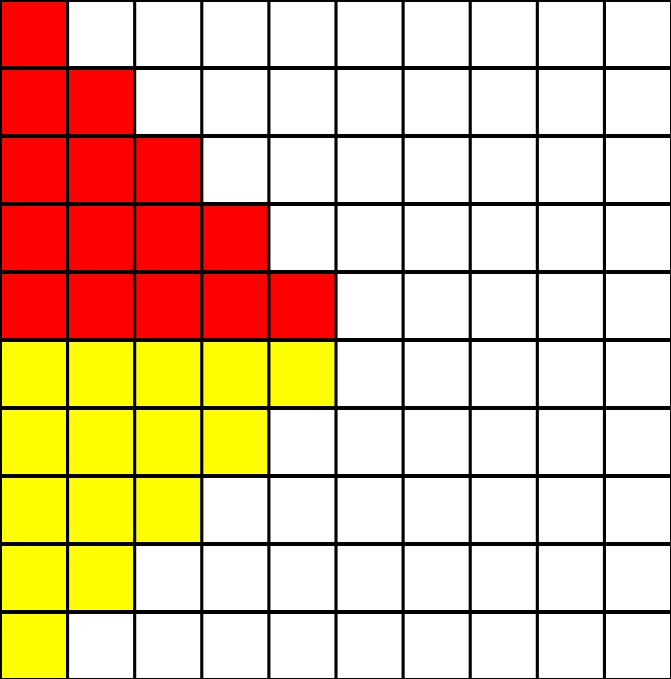
\includegraphics[scale=0.25]{symmetries.png}\\
The red area shows the 8-way symmetric region. The red and yellow region together constitute the 4-way symmetric region.
\end{center}
\section*{\emph{\textmd{Piece Stability}}}
\hrule

A given board tile is stable if it is impossible for it to ever be taken. This is very important as it reduces opponent's opportunities to flip tiles and puts the player in a good position to influence the board. Stability is especially important in this Othello variant as the blocked squares can significantly increase the number of stable tiles. 

A piece position is stable if the 4 directional axes (North-South, East-West, NW-SE, NE-SW) are all stable. A directional axis is stable if$^{[3]}$
    \begin{itemize}
\item The axis is 'full' - travelling along the lines on this axis on both sides of the piece position, we hit the end or a blocked square before finding any empty slots.
\item One of the neighbouring squares along each axist is stable and the same colour.
\end{itemize}

This is because pieces cannot be captured along full axes, and if a neighbour can't be taken, there is no possibility to 'get behind' that piece to take it (at least along that axis).

\begin{center}
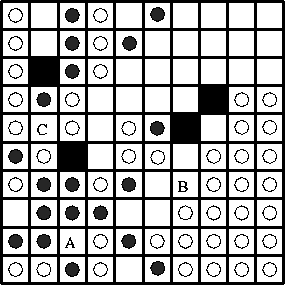
\includegraphics[scale=0.50]{stability.PNG}\\
Stable positions for white
\end{center}

Stability is a relatively expensive check because determining the stability of one piece requires testing a considerable number of points along the board. Complete board checking requires testing every single nonempty position. Additionally, since piece stability can depend on nearby pieces, to accurately find all stable positions we need to loop through the entire board until we find no new stable positions. This checking greatly slows down the search speeds, which became an issue due to the time constraints of the problem.

Stability memory was implemented in order to decrease the cost of computing stable nodes. Exploiting the fact that once a position is stable, it is always stable, we can keep track of the pieces that have already been found to be stable, and update this as we move. This avoids the need to repeatedly do an expensive complete board stability check. While overall this requires more computation from root game tree node to leaf, it moves the computation up as far in the game tree as possible, so that the computation is done once and shared along all the branches rather than being fully computed at each leaf node.

At the start of every move decision, the root node's complete board stability is checked. As each possible move is expanded, the stability of that move is checked. If that move fills any directional axes, the directional axes that were filled are checked. The results are saved in a stability matrix, and passed down the game tree. This greatly reduces total computation required.

It should be noted that this method is not complete, only a largely accurate estimate. There are less common circumstances where this algorithm gives false negatives. If a piece is made stable only by the stability of a point along the axis, it may not be found to be stable.

To fix this, we could test all pieces in all directions of a move, and then if we find any stable positions, retest all the directions from the stable positions. However, the increased computation required would outweigh the benefits of the gain in accuracy.

\begin{center}
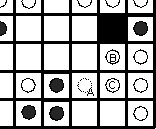
\includegraphics[scale=0.6]{falsepos.PNG}\\
If white moves in position A, the algorithm will detect that B is stable\\ but will fail to test the stability of C as it is not on a full line.
\end{center}

    \begin{itemize}
  \item
    Importance gets diluted in late game because in late game, EVERYTHING is stable. this is a consequence of only using 3 phases
  \end{itemize}
\section*{\emph{\textmd{Mobility}}}
\hrule

Mobility is the number of moves a player has in a given board state. High mobility increases the number of options available to a player, increasing the change they have a good move, and that they can out-position their opponent. Low mobility can reflect a poor position with a lack of options, and lead to forced moves.

Mobility tends to be the strongest predictor of a good position during the early game. In the mid and late game, it is less favoured than stability and control of the corners, but otherwise is still a strong predictor of the value of a position.

It also has the unfortunate side effect of increasing the branching factor in the MinMax search, to the point where the increased number of available moves can mean we have to search to a lesser depth.
\section*{\emph{\textmd{Piece Internality}}}
\hrule

A piece is internal if it has no empty neighbours. This can be a useful indicator of a player's position on the board. While it can be useful sometimes, as internal pieces can also be harder to dislodge, the strategy learnt by the agent favoured less internal pieces and imposed a penalty on them.

This is computationally cheap to check. Exploiting the fact internal pieces stay internal even if they are flipped, partial memory of internality was also used (internality checked and remembered for every new move).

\begin{center}
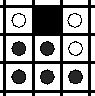
\includegraphics[scale=0.50]{internality.PNG}\\
The centre piece is an internal node.
\end{center}
\section*{\emph{Temporal Difference Learning}}
\hrule

Our learning algorithm is based on TD($\lambda$), although we do not implement that algorithm exactly.

When learning is enabled, we play through the entirity of a game, storing each board position. At the end, we recieve a reward equal to the difference in the number of pieces for each player in the terminal state.

Then, for each board $b_k$, and for each feature weight $W_f$, we choose which direction to adjust the weight in by making a small change in the value of the weight, and determining whether that would improve or worsen the value of the board. The point here is that we are calculating an approximation of the gradient of our evaluation function $V(b)$ at $b_k$, with respect to the feature $W_f$: $\frac{\Delta V(b_k)}{\Delta W_f}$, thus allowing us to perform gradient descent.

We then run through each successor $b_t$ of $b_k$, and calculate the difference between the value of $b_t$ and $b_k$, weighted by some discount factor $\gamma^{t-k}$.

Finally, the value of the feedback is also added in, weighted by the distance from $b_k$ to the terminal board $b_K$.

More formally, we calculate 
\begin{eqnarray}
	W_f  & \leftarrow & W_f + \alpha \frac{\Delta V(b_k)}{\Delta W_f} \nonumber  \\
	&&  \times \left(\gamma^{K-k}r + \sum_{t=k+1}^K \gamma^{t-k}\left(V(b_t) - V(b_k)\right)\right) \nonumber
\end{eqnarray}

Where
   \begin{itemize}
  \item
  	$W_f$ is the weight of feature $f$,
  \item
	$V(b_i)$ is the value of a board $b_i$,
  \item
	$r$ is our reward,
 \item
	$\alpha$ is our learning rate,
  \item
	$\gamma$ is our discount factor, and
  \item
	$K$ is the index of the terminal board.
  \end{itemize}

Values of $alpha = 0.0001$ and $\gamma = 0.9$ were used during our learning process.

To try and balance the exploration vs exploitation problem that is so frequently found in temporal difference learning, we utilised an $\epsilon$-greedy policy, whereby the agent would select a random move 15\% of the time, and an optimal (in the sense of its estimate of the value of a board state) move 85\% of the time.
\section*{\emph{\textmd{Learning Results}}}
\hrule

\begin{center}
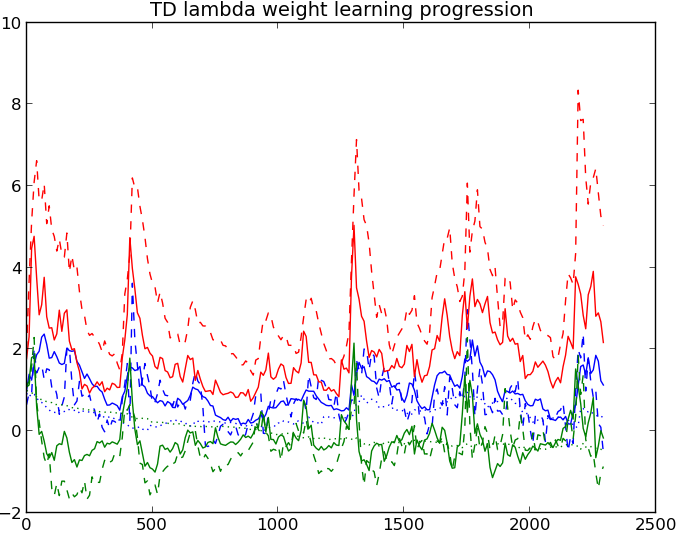
\includegraphics[scale=0.40]{longgraph.png}\\
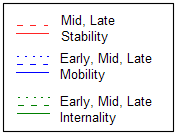
\includegraphics[scale=0.50]{legend.PNG}\\
Feature weight learning over 2300 games of self-learning
\end{center}

We can see from the above graph that the weights learnt are clearly not converging. This is most likely due to the fact that the weights are not independant of each other: stability, mobility and internality all affect each other to a degree, and as their importance adjusts, and boards utilising these features become more prominent, it causes the importance of other weights to adjust as well. The stochasticity of the domain (random blocked squares) together with the $\epsilon$-greedy algorithm used in TD also impede convergence.

The learning seems to oscillate between calmer areas where the are only minor changes to the weights, followed by brief periods with a high degree of volatility in the weights. The 'calm' areas are likely to respond to the more considered strategies, such as the weights learned at about game 850 or game 2070.

The above graph is slightly misleading, as because the feature weights are all relative, direct comparisons between early, mid and late game weights should not be made, but comparisons about the relative importance of weights within each set can be made.

The weights at game 2070 are as follows:
\section*{\emph{\textmd{Early Game}}}
\begin{tabular}{| l | l | l | l | l | }
\hline
 0&&&&\\
\hline
 0& 7.48E-6&&&\\
\hline
 0& 2.18E-5&-1.70E-4&&\\
\hline
 0& 1.11E-5&-2.67E-4&-1.60E-4&\\
\hline
 0&-4.56E-5& 1.21E-4& 1.64E-4& 2.00E-4\\
\hline
\end{tabular}
\medskip{}\\
Mobility Weight: 3.16E-1\\
Stability Weight: 0.00000E+0\\
Internality Weight: -4.00E-1
\section*{\emph{\textmd{Mid Game}}}
\begin{tabular}{| l | l | l | l | l | }
\hline
 2.80513E+0&&&&\\
\hline
 3.73E-1&-2.56E-3&&&\\
\hline
 3.20E-3&-1.56E-4& 1.27E-3&&\\
\hline
-1.00E-5&-5.23E-4&-1.56E-3& 4.79E-4&\\
\hline
 1.14E-3&-5.52E-4& 4.10E-4& 7.66E-4& 2.00E-4\\
\hline
\end{tabular}
\medskip{}\\
Mobility Weight: 3.79E-1\\
Stability Weight: 2.33893E+00\\
Internality Weight: -3.51E-1
\section*{\emph{\textmd{End Game}}}
\begin{tabular}{| l | l | l | l | l | }
\hline
 2.25830E+0&&&&\\
\hline
 1.12976E+0& 2.20E-4&&&\\
\hline
-2.79E-4&-3.39E-4& 7.21E-4&&\\
\hline
 4.53E-4& 3.78E-4&-3.29E-4& 1.89E-4&\\
\hline
 5.14E-4& 2.86E-4&-7.56E-5& 1.22E-4& 2.55E-6\\
\hline
\end{tabular}
\medskip{}\\
Mobility Weight: 5.12E-1\\
Stability Weight: 1.45929E+0\\
Internality Weight: -2.81E-1
\section*{\emph{Negamax with alpha beta pruning}}
\hrule

Negamax is an adversarial search algorithm which expands the game tree in a depth first search in order to maximise game value, under the assumption that the opponent, who makes the same assumptions about game value, is trying to minimise that value. This is achieved in a simple recursive fashion by recursively calling negamax and negating the values at each step.$^{[4]}$

The alpha-beta pruning extension allows us to disregard branches of the game tree that a player would not give the opponent a chance to play (because it is too good for their opponent), significantly reducing the size of the game tree that needs exploring.

Negamax is very useful as it emulates a game play environment, where while we moving the board into a good state for us, the opponent is actively trying to move to make the board a worse state for us.

The major disadvantage of Negamax is the assumption that the opponent values each board exactly the same way as we do. This is especially problematic with alpha beta pruning - we may prune states which very good moves based on the assumption that the opponent will never let us play those moves, but in real play, the opponent might let us play those moves if they don't see the value.
\section*{\emph{\textmd{Negamax Implementation}}}
\hrule

Because the entire game tree isn't computable, our negamax has a depth cutoff. A small (but useful) optimisation to this process is increasing the search depth by 1 if we explore along a forced move - both because there is no branching that would increase computation cost, and this is an interesting board that we should explore further.

At the cutoff, the agent uses the static evaluation function in order to determine the degree to which the board state is (or is not) in our favour.

At terminal states, the board is evaluated to be -$\infty$ if we lose, or +$\infty$ if we win. This encodes the fact that any win is equal, regardless of the piece margin, and we should prioritise an outright win, and also that any loss is equal and should be avoided at all costs.

The advantages are that we will take a guaranteed opportunity to wipe out the opponent early, or at the end of the game, move towards a safe guaranteed win rather than trying for a win with the most pieces. However the disadvantage is if we see that a perfect opponent would cause us to lose no matter how well we play, the agent surrenders and plays the first move it sees, rather than attempting to minimise the loss margin in the hope that the opponent makes a mistake and allows our victory.

In normal play, the agent searched to a depth of 7 in the game tree (see Time Management). Once the end of the game was within sight (12 moves left on the board), the depth was increased to allow the entire game tree to be evaluated. This allowed us to make perfect play (and at this point, we could determine whether we would win or lose to a perfect player).
\section*{\emph{Concurrency}}
\hrule

We utilised concurrency to reduce the amount of time taken to do a MinMax search to a fixed depth. This involved splitting the workload of computing the search tree between a number of worker tasks, typically equal to the number of CPU cores available to use for computation.

In doing so, we had to find a model of parallelism which balanced what was theoretically an optimal way of parallelising the computation, with the reality that any model of parallelism involves at least some overhead in communication between tasks, and in waiting on access to shared data structures.

The first model considered was one in which the root node of the MinMax search tree is pushed onto a stack, and then the worker nodes pop from this stack, expand the node which they popped, and push the resulting list back onto the stack. The result would be an approximately-depth-first search, and is \begin{em} theoretically \end{em} a very nice model of parallelism, since worker time is assigned where it is actually needed. However, there is the potential for significant overhead in writing to the stack (especially as Ada has a habit of copying variables instead of referencing them), leading to long waiting times for accessing it. There is also a not inconsiderable amount of overhead involved in tracking alpha-beta values and the best values for particular moves, which would make implementing this model challenging.

We therefore settled on a second, more straightforward method of parallelising the computation. In this model, the worker threads poll a central data structure in order to recieve a node to evaluate. This node corresponds to one of the Min nodes which are direct successors of the root Max node in the MinMax search tree. The node is then evaluated in full (to the specified fixed depth) and without communication with either the other workers or the central data structure. Once evaluated, the results (i.e the value of that move) are reported to the central data structure, which aggregates the results. The worker then requests a new node to evaluate, and the process repeats.

\begin{center}
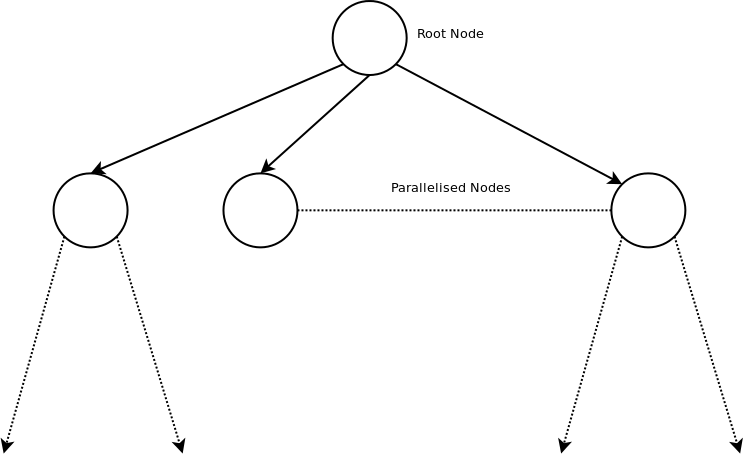
\includegraphics[scale=0.31]{concurrency.png}
\\Concurrency model
\end{center}

This model has the advantage of having very little overhead in terms of communication, and a relatively low chance of two worker tasks trying to simultaneously access the data structure (at least after the first batch of nodes is given out). The downside is that there is no consideration given to the amount of resources (i.e. worker time) needed to evaluate a node - the same amount of resources are allocated regardless of whether the node is a terminal, or a full search tree with a large branching factor. In practice however, this is not a significant problem, as if one node is evaluated quickly, the worker will simply be assigned another one.

One issue that does arise with this model is that the first node (or first set of nodes) evaluated almost always takes the longest amount of time, when compared with the other nodes. This appears to be true regardless of the number of workers assigned to the task. Our theory as to the reason behind this is that, for the first nodes, we do not have accurate $\alpha\beta$ values when exploring the tree, so much more will tend to be explored than is strictly necessary. Once at least one of the initial nodes returns, and its information aggreated into the central data structure, all subsequent nodes will be evaluated with at least the $\alpha\beta$ values of that first node, allowing for much more efficient pruning.

The results of our parallelism is an $O(n)$ speed-up in computation time, where $n$ is the number of cores we are using. In practice, this gave us an extra one to two levels of MinMax search, running on a 4-core machine.
\section*{\emph{Time management}}
\hrule

A simple rule system was used to manage the time limitations imposed. The depth of the search was adjusted according to how much time we had left, how difficult the previous move was to compute, and how far we had until the end of the game.

As emergency mechanisms, if the agent had 15 seconds left, it searched to depth 4. If the agent had only 5 seconds left, it searched to depth 2.

If there was less than 30 seconds available, or the previous move took a long time to compute (likely indicating a large branching factor), the agent searched to depth 5 to conserve time.

If there was more than 50 seconds available, and the previous move took a short time to compute (indicating a lower branching factor that we can search deeper into), the agent searched to depth 5.

Otherwise, the agent defaulted to the normal depth of 7.

This system was simple yet able to respond to different scenarios without forfeiting on time, whilst utilising most of the time available.

However, the downside of such a simple system is that the agent did not respond to time constraints mid-search. In an extreme scenario, with 31 seconds left, the agent may attempt its normal search depth on a board with a huge branching factor and take longer than the remaining time. This could be avoided by checking the timing mid-computation and breaking off to employ emergency mechanisms if required.
\section*{\emph{C++ and Ada}}
\hrule
A mix of C++ and Ada code was used for the agent. C++ listened for and recorded server messages, and Ada was used for the main computation. This was effective in playing to the advantages of both languages. C++ was able to handle the server messages on a bit level, whereas this is more difficult for Ada as it is very strongly typed. On the other hand, Ada is very well suited for concurrent computation and this was used in order to fully utilise available hardware (see \emph{Concurrency}.

At all times there were at least two threads. The main function in C++ listened for server messages, and a persistent task in Ada waited for instructions from C++.

C++ called three Ada procedures, which in turn called entries (synchronisation constructs) on Ada's main task. Initialise set the initial player colour and loaded weights, NextMove asked Ada to choose a move and EndGame asked Ada to learn then terminate.

Shared memory structures were used to pass information between C++ and Ada. Contention was avoided by ensuring either C++ or Ada was blocked at all times, which guaranteed mutual exclusion.

The main function in C++ was used to facilitate network communications, from the sample client code. C++ then called the appropriate functions in Ada.

\section*{\emph{Other ideas (Monte Carlo)}}
\hrule
A Monte Carlo function may be used to predict the likelyhood of wining, based on a random sampling of possible end board states arising from the one being currently evaluated. This has a number of practical uses in the Othello problem:

Firstly, it can be utilised in conjunction with MinMax in order to differentiate moves which are likely to be good. The process would involve selecting (for example) the 10 best boards from a MinMax search to some fixed depth, and then performing Monte Carlo sampling of the end-boards from each of these positions. This would provide a probability of winning from each of those board positions, which we could then use to weight the values returned for each board by the static evaluation function, giving us a final value.

The advantage of this technique is that it provides a concrete approximation to the likelyhood of winning from a given board position. Indeed, given a large enough level of sampling, Monte Carlo could potentially replace MinMax altogether.

The other potential use for Monte Carlo is as an approximation to the reward used in the temporal difference learning algorithm. Here we again sample the end board states that arise from a given board state, and use this probability of winning as the reward value for a particular state. This allows us to get around the problem we encounter in Othello (and other similar board games) in that we only know the outcome of the game at the very end, thus alowing us to learn on-the-fly, instead of at the end of every game. This presumably would allow us to learn accurate feature weights more quickly.

At one point in the development of our agent, we had implemented parts of both of these ideas. However, Monte Carlo was re-replaced with MinMax for our search function, as it was not performing particularly well (at least not for the sample sizes we were using), and it's use as a reward approximator was removed, as at that time the temporal difference learning function was not behaving as desired, and it was neccessary to try and remove any points of possible error.

\section*{\emph{Other ideas (NegaMax)}}
\hrule

Several possible further optimisations to negamax searching were considered.

By optimising the order in which we explored nodes to search the most promising boards first, we could have greatly increased the amount of pruning. This can also be difficult as the ordering needs to be simple, otherwise the benefit of the optimised ordering becomes outweighed by cost to compute the ordering.

A considerable amount of time could be saved by storing the results of searches in between moves, and continuing on from the results of previous computations (after pruning the now irrelevant game trees considered). An approach achieving a similar function would be to store a transition table of states previously considered. Additionally, a considerable amount of computation time could be gained by utilising time while the opponent is thinking. However all of these possibilities would have required extra memory management and data structures and the extra complication would have made concurrency more difficult.

A variable search depth, based on the branching factor and volatility of the state (possibly corresponding to a really good move) could also have improved the search considerably.
\section*{\emph{Other ideas (Evolutionary Algorithm)}}
\hrule
    \begin{itemize}
  \item
   	Use an evolutionary algorithm strategy to play agents off against each other.
  \item
	Use feature values as 'genes'.
  \item
	'Breeding' via exchanging features. Don't need a heuristic for which to exchange, as features tend to be relatively independent.
  \item
	Mutation via small random change to a feature.
	\\ e.g. from a uniform distribution around (-1,1), or
	\\ Normal distribution with mean 0.
  \item
	Essentially still doing gradient decent. Can be used as a substitute for an $\epsilon$-greedy policy.
  \end{itemize}
  
\section*{\emph{References)}}
\hrule

[1]
Stephen Gould\\
\emph{Othello Project (Handout $\#$3)} (s2012)\\
  
[2] Yasuhiro OSAKI, Kazutomo, SHIBAHARA, Yasuhiro TAJIMA, Yoshiyuki KOTANI\\
\emph{An Othello Evaluation Function Based on Temporal Difference Learning using Probability of Winning} (2008)\\
$<$http://www.csse.uwa.edu.au/cig08/Proceedings/papers/8010.pdf$>$

[3]
Amy S. Biermann\\
Stability, \emph{Othello implementation} (1994)\\
$<$http://www.pressibus.org/ataxx/autre/minimax/node3.html$>$

[4]
Wikipedia\\
\emph{Negascout} (2012)\\
$<$http://en.wikipedia.org/wiki/Negascout$>$
\end{multicols}
\end{document} 
